\documentclass{article}
\usepackage{graphicx}
\usepackage{amsfonts}
\usepackage{amsmath}
\usepackage{url}
\usepackage{subcaption}
\usepackage[left=3cm,top=3.0cm,right=3cm,bottom=3.0cm]{geometry}


\newcommand{\norm}[1]{\left\lVert #1 \right\rVert}
\title{Accuracy of Newton-Krylov for Particle Methods}
\author{Hannes Vandecasteele}
\date{May 2025}

\begin{document}

\maketitle

\section{Newton-Krylov for Steady States of Timesteppers}
\subsection{Introduction}
Let 
\begin{equation} \label{eq:pde}
    \partial_t x_t = f\left(x_t\right)
\end{equation}
be a semi-discretized PDE. We are interested in steady-state points $x^*$ such that $f(x^*)=0$. However, in most codes the right-hand side $f$ of the PDE is not directly available. It is implicitly encoded in a timestepper subroutine. Denote by $\phi_T(x)$ the flow map of a timestepper with initial condition $x$ over a time interval of size $T$. Then, by definition, 
\begin{equation*} 
    \phi_T(x) = x_T.
\end{equation*}
Steady-state profiles of the PDE~\eqref{eq:pde}, i.e. zeros of $f$, must also satisfy
\begin{equation}
    \psi(x) = x - \phi_T(x) = 0
\end{equation}
because a steady state $x$ indicates that it remains unchanged after applying the timestepper. By design, the function $\psi$ is always available because it is based on a timestepper subroutine. Furthermore, stable steady states of $f$ are stable steady states of $\psi$ and vice versa. Finally, the characterization of a steady state remains unchanged because eigenvalues $\lambda_i$ of $f$ are related to the eigenvalues $\mu_i$ of $\psi$ through
\begin{equation}
    \mu_i = 1 - \exp\left(-T \lambda_i\right).
\end{equation}
The eigenvectors remain the same. I have a separate document containing proofs of these facts.

\subsection{Finite Differences and the Newton-Krylov Method}
A straightforward way to actually compute the zeros of $\psi$ (steady states of the PDE) is by the Newton-Raphson method. The main idea behind Newton's method is to build a sequence of successive approximations $\{x_k\}_{k=1}$ to the steady-state solution $x^*$ through the updating formula
\begin{align} \label{eq:newton_system}
    J(x_k) s_k &= -\psi(x_k) \\
    x_{k+1} &= x_k + s_k.
\end{align}
Newton's method is guaranteed to converge to $x^*$ as long as the initial condition $x_0$ is chosen well. However, in many practical implementations, the Jacobian $J(x_k) = D\psi(x_k)$ is not available in code. Instead, we approximate actions of the Jacobian $J(x_k) v$ using finite differences
\begin{equation} \label{eq:fd}
    J(x_k) v \approx \tilde{J}(x_k) v = \frac{\psi(x_k + \varepsilon v) - \psi(x_k)}{\varepsilon}
\end{equation}
where $\varepsilon$ is the finite-differences step size. Then, we must solve~\eqref{eq:newton_system} using a Krylov method (often GMRES or L-GMRES) because the Jacobian is only known through its actions on vectors. Technically, we solve a modified system
\begin{align} \label{eq:newton_system_mpd}
    \tilde{J}(x_k) \tilde{s}_k &= -\psi(x_k) \\
    x_{k+1} &= x_k + \tilde{s}_k.
\end{align}
due to the approximation error in the finite differences scheme.

\subsection{Accuracy of Newton-Krylov}
By applying the finite differences approximation to the Jacobian, we will always make approximation and rounding errors. It can be proven that the combined error is $\mathcal{O}(\varepsilon)$ for $\varepsilon \approx 10^{-8}$, i.e.,
\begin{equation}
    \tilde{J}(x_k) v = J(x_k) v + \mathcal{O}(\varepsilon).
\end{equation}
How does this approximation error affect the accuracy of Newton-Krylov? Said differently, how close can Newton-Krylov get numerically to the true steady state $x^*$? 

A key result from a somewhat forgotten paper~\cite{dembo1982inexact} states that the maximal accuracy is essentially determined by the condition number of the root $x^*$ of $\psi$, given by 
\begin{equation}
    \kappa(x^*)= \norm{J(x^*)^{-1}}
\end{equation}
This condition number also fundamentally determines the accuracy of the Newton method. Let $r_k$ be the residual of the solution $s_k$ of the linear system~\eqref{eq:newton_system_mpd} after solving it with a Krylov method. This residual is defined as
\begin{equation} \label{eq:residual}
    r_k = J(x_k) \tilde{s}_k + \psi(x_k)
\end{equation}
The residual error contains two components: 1) The approximation error $\mathcal{O}(\varepsilon)$ in the Jacobian $\tilde{J}$, i.e. the fact that we're solving the wrong system with matrix $\tilde{J}$ instead of $J$; and 2) the tolerance $\delta$ that is typically used to stop Krylov solvers. So after the linear system solver converges, we have the guarantee that $\norm{r_k} \leq \delta$ for all $k$. Combining these, we find
\begin{equation}
    \norm{r_k} = \norm{J(x_k) \tilde{s}_k + \psi(x_k)} \leq \delta + C \varepsilon
\end{equation}

The paper states two main results.
\begin{itemize}
\item[1.] If the forcing sequence $\eta_k = \norm{r_k} / \norm{\psi(x_k)}$ decreases to zero, then the Newton method converges superlinearly; 
\item[2.] If $\eta_k$ is uniformly less than one, the `converged' error $\norm{x_{\infty} - x^*}$ is bounded above by 
\begin{equation*}
    \norm{J(x^*)^{-1}} \max_k \norm{r_k}.
\end{equation*}
This is a strong result and mainly due to the quadratic convergence behavior of the  Newton method.
\end{itemize}

Applying these results to our setting, we find that the Jacobian-free Newton-Krylov method can reach the true steady-state solution $x^*$ up to an error given by
\begin{equation} \label{eq:nk_accuracy}
    \norm{x_{\infty} - x^*} \leq \norm{J(x^*)^{-1}} \max_k \norm{r_k} \leq \norm{J(x^*)^{-1}} \left(\delta + C \varepsilon\right)
\end{equation}
Here, $C$ is the proportionality constant in the finite differences approximation error.

\subsection{On Choosing $T$ and the Signal-to-Noise Ratio}
I know how to do it for symmetric matrices, because then the Jacobian $M(x_k)$ of the \textbf{timestepper} $\phi_T$ can be decomposed as
\begin{equation}
    M(x_k) v = \sum_{i=1}^n \exp(-T \lambda_i) v_i v_i^T v
\end{equation}
where $v_i$ are the eigenvectors. Note that $J(x_k) v = v - M(x_k)v$. When the eigenvalues are ordered, i.e., $|\exp(-T \lambda_i)| > |\exp(-T \lambda_j)|$ for $i < j$, then this expansion can be rewritten as the dominant term plus high-frequency corrections
\begin{equation}
    M(x_k) v =  \exp(-T \lambda_1)v_1 v_1^T v + \sum_{i=2}^n \frac{\exp(-T \lambda_i)}{ \exp(-T \lambda_1)}v_i v_i^T v.
\end{equation}
For a high signal-to-noise ratio, we want 
\begin{equation}
    \frac{\exp(-T \lambda_i)}{\exp(-T \lambda_1)} \ll 1
\end{equation}
and this provides a criterion for choosing the minimal integration time $T$. Defining the signal-to-noise ratio as $\eta$ with $1/\eta \ll 1$, we want that
\begin{equation*}
    \exp\left(-T(\lambda_i - \lambda_1)\right) \leq \frac{1}{\eta}
\end{equation*}
 for all $i > 1$, and therefore
\begin{equation}
    T \geq \frac{\ln \eta}{|\lambda_1 - \lambda_2|}
\end{equation}
Remember that $\lambda_i$ are the eigenvalues of the right-hand side of the PDE~\eqref{eq:pde} and they all have a negative real part in the stable regime. In practice, we have to choose a value of $\eta$ and then the minimal integration time window will essentially depend on the gap of the eigenvalue distribution.

It is an open question how much of this analysis carries over to the non-symmetric case.

\section{Newton-Krylov for the Fokker-Planck Equation}
The end goal of this project is to apply our matrix-free Newton-Krylov framework to particle methods. As this setup is not well-defined (see the next section), we decided to look at the steady-state distribution of the Fokker-Planck equation first. Let $X_t$ be a random variable given by the SDE
\begin{equation}
    dX_t = \mu(X_t, t) dt + \sigma(X_t, t) dW_t.
\end{equation}
The evolution of the probability density function $p(x, t)$ of $X_t$ is determined by the Fokker-Planck PDE
\begin{equation}
    \partial_t p(x,t) = -\partial_x \left(\mu(x,t) p(x,t)\right) + \frac{1}{2}\partial_{xx} \left(\sigma^2(x,t) p(x,t)\right)
\end{equation}
Obviously, steady states of the SDE coincide with steady-state distributions of the Fokker-Planck equation. However, since the FP equation is fully deterministic, we can directly apply a Newton-Krylov method to find these steady states. We have done this on three examples: the overdamped Langevin equation with a bimodal potential, a simple chemotaxis model, and an advanced chemotaxis model. We report our findings in the three sections below.

\subsection{Langevin Equation with a Bimodal Potential}
The first example is a simple bimodal distribution given by the potential energy
\begin{equation} \label{eq:bimodal_potential}
    V(x) = \frac{1}{2}\left(x^2 - 1\right)^2
\end{equation}
The associated overdamped Langevin dynamics and Fokker-Planck equation read
\begin{align}
    dX_t &= -\nabla V(X_t)dt + \sqrt{2} \beta^{-1} dW_t \\
    \partial_t p(x,t) &= \partial_x \left(\nabla V(x) p(x,t)\right) + \beta^{-2} \partial_{xx} p(x,t)
\end{align}
In our notation, $\beta = (k_B T)^{-1}$ is the inverse temperature and we fix it to $\beta=2$. The invariant distribution is given by the Boltzmann-Gibbs distribution and reads
\begin{equation}
    p(x) = p(x,t=\infty)= Z^{-1} \exp\left(-\beta V(x)\right)
\end{equation}
where $Z$ is the normalization constant.

To compute this steady-state distribution, we applied Newton-Krylov to a simple Euler + finite differences timestepper that integrates the solution over a time window of $T = 0.1$ seconds with a time step of size $\delta t = 10^{-5}$. The spatial grid consists of $1000$ grid points. Our finite differences timestepper uses central differences for the diffusion term, and upwind/downwind for the advection term depending on the sign of the drift. The final result is shown in Figure~\ref{fig:bimodal}.
\begin{figure}[ht]
    \centering
    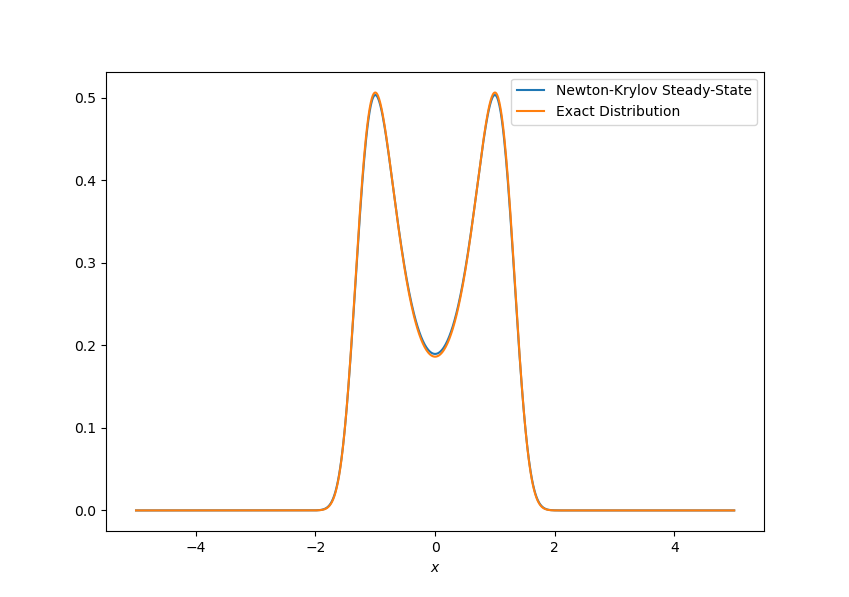
\includegraphics[width=0.8\linewidth]{figures/Bimodal Steady State.png}
    \caption{Invariant distribution found by Newton-Krylov (blue) and the Boltzmann-Gibbs distribution (orange) for the bimodal overdamped Langevin dynamics.}
    \label{fig:bimodal}
\end{figure}
One can see that we fully recover the Boltzmann-Gibbs distribution! Even more, the Newton-Krylov optimizer fully converged to machine precision with a residual (i.e. value of $\psi$) of less than $10^{-15}$!

Secondly, we also employed the Arnoldi method to compute the leading eigenvalues (those closest to $1$, or the ones of largest magnitude) of the timestepper. They are shown in Figure~\ref{fig:bimodal_eigenvalues}.
\begin{figure}[ht]
    \centering
    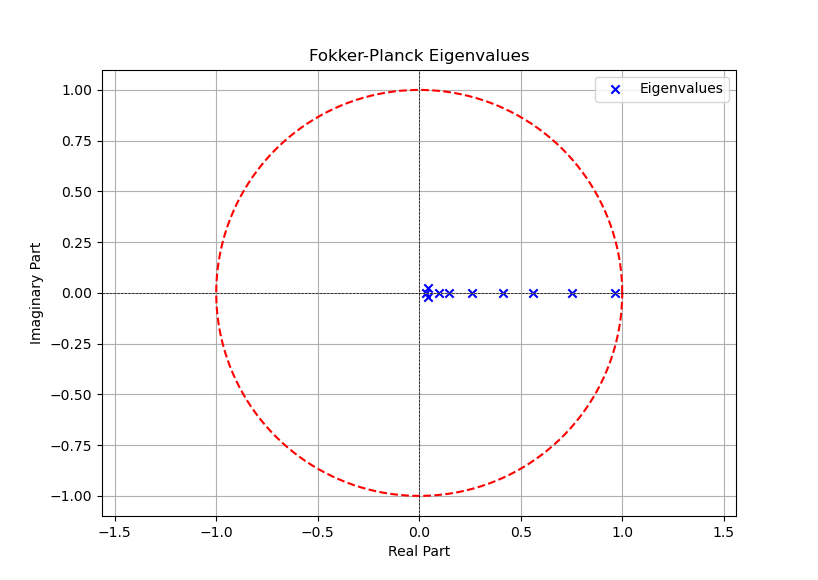
\includegraphics[width=0.8\linewidth]{figures/Bimodal Eigenvalues.png}
    \caption{Eigenvalues (blue crosses) of the Fokker-Planck timestepper}
    \label{fig:bimodal_eigenvalues}
\end{figure}

\subsection{A Simple Chemotaxis Model}
The second example is a simple chemotaxis model. Let $X_t$ be the random positions of bacteria at time $t$. The function $S(x)$ represents the food source at position $x$, and we assume that the amount of food remains unchanged. Think of this model as being linked to a separate but unspecified process that replenishes the food. Furthermore, there also is a chemotactic sensitivity $\chi(S)$ that is solely a function of the local food supply. Finally, we also incorporate a diffusion constant $D$ to model the random movements of the bacteria. The Langevin dynamics for the bacterial positions reads
\begin{equation}
    dX_t = \chi(S(X_t)) S_x(X_t) dt + \sqrt{2D} dW_t
\end{equation}
where $S_x = \partial_x S$ is the food gradient. This Langevin process models bacteria moving to areas with greater food supply as well as random noise. The associated Fokker-Planck equation is
\begin{equation}
    \partial_t \mu(x,t) = -\partial_x\left(\chi(S(x)) S_x(x) \mu(x,t)\right) + D \partial_{xx} \mu(x,t).
\end{equation}
The advantage of this simple model is that we can derive an analytic formula for the steady-state distribution. It can be shown (using ChatGPT - I am not a mathematician) that 
\begin{equation} \label{eq:chemotaxis_ss}
    \mu(x) = \mu(x,t=\infty) = Z^{-1} \exp\left(\frac{1}{D} \int_{0}^{S(x)} \chi(S) dS\right)
\end{equation}
where $Z$ is again a normalization constant.

In the following numerical example, we use $S(x) = \tanh(x)$ and $\chi(S) = 1 + \frac{1}{2}S^2$. We employ a simple Euler timestepper with step size $\delta t = 10^{-3}$ and a finite-differences discretization in space (central for diffusion, upwind/downwind for advection). The domain is $[-10, 10]$.

In Figure~\ref{fig:simple_chemotaxis_ss}, we show the Newton-Krylov invariant distribution by integrating the timestepper over $T = 1$ second. We also show the analytic invariant distribution and see a perfect match! Newton-Krylov again converged to machine precision (on $\tilde{J}$ of course, not $J$). We also show the Arnoldi eigenvalues in Figure~\ref{fig:simple_chemotaxis_arnoldi} 
\begin{figure}[ht]
    \centering
    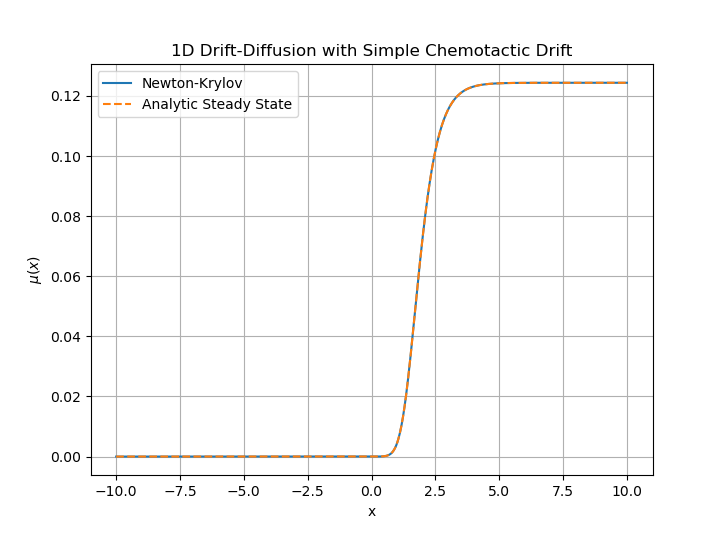
\includegraphics[width=0.8\linewidth]{figures/Simple Chemotaxis Steady State.png}
    \caption{Steady-state distribution of the simple chemotaxis model. Orange is the analytic steady state given by equation~\eqref{eq:chemotaxis_ss}, while blue is the numerical steady-state profile obtained by Newton-Krylov.}
    \label{fig:simple_chemotaxis_ss}
\end{figure}

\begin{figure}[ht]
    \centering
    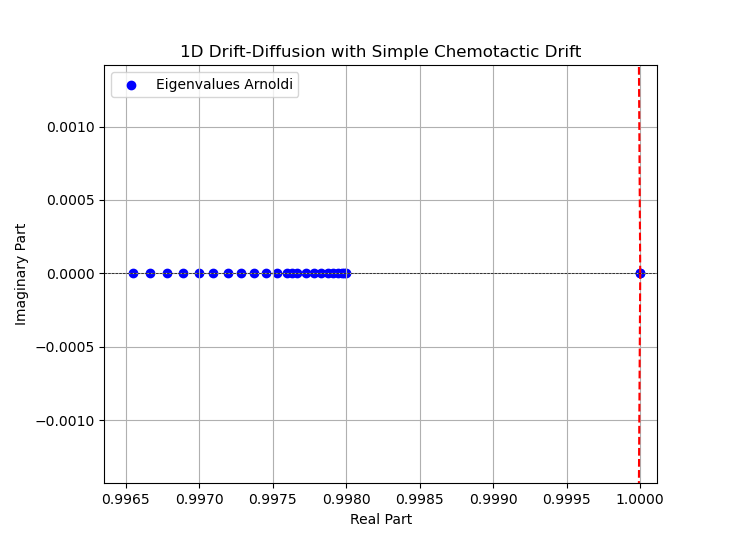
\includegraphics[width=0.8\linewidth]{figures/Simple Chemotaxic Eigenvalues.png}
    \caption{Arnoldi eigenvalues of the simple chemotaxis model. These eigenvalues are all very close to one and very clustered, so not sure if they are correct, but everything else looks find numerically.}
    \label{fig:simple_chemotaxis_arnoldi}
\end{figure}

\subsection{An Advanced Chemotaxis Model}
As a final example, we consider a much more advanced bacterial chemotaxis model. The Fokker-Planck PDE reads
\begin{equation}
\frac{\partial B}{\partial t} = D_B \frac{\partial^2 B}{\partial x^2} - \frac{\partial}{\partial x} \left[ \frac{\chi_0}{1 + B/B_h} B \frac{\partial}{\partial x} \ln(1 + A(x)/K_i) \right]
\end{equation}
The food source function $A(x)$ is a scaled Gaussian with zero mean and a standard deviation of $50$, 
\begin{equation*}
    A(x) = \exp\left(-\frac{1}{2}\frac{x^2}{50^2}\right)
\end{equation*}
The other parameter values are $D_B = 440$, $\chi_0 = 3800$, $B_h = 6.8$ and $K_i = 1$. The domain is $[-500,500]$.

There is a particle SDE associated with this equation, but it is of McKean-Vlasov type where the density $B(x,t)$ appears directly in the drift term, so we need to co-evolve the particles and its density. These problems don't appear when we just solve for the steady state of the Fokker-Planck PDE. To my knowledge, the above PDE does not have an analytical steady state, so we can only compute it numerically through time evolution or using Newton-Krylov.

We again use a simple Euler timestepper with time steps of size $\delta t = 10^{-3}$. We use a finite differences discretization in space with $1001$ grid points. Again, central differences for the diffusion and upwind/downwind for the advection depending on the sign of the drift term. For Newton-Krylov, we integrate the timestepper for $T = 1.0$ seconds. Figure~\ref{fig:advanced_chemotaxis_ss} shows the steady-state distribution obtained through both time evolution up to $T = 1000$ seconds and Newton-Krylov. We can see that both distributions match up to machine precision (in terms of $\psi$). Furthermore, the Arnoldi eigenvalues are depicted in Figure~\ref{fig:advanced_chemotaxis_arnoldi}.

\begin{figure}[ht]
    \centering
    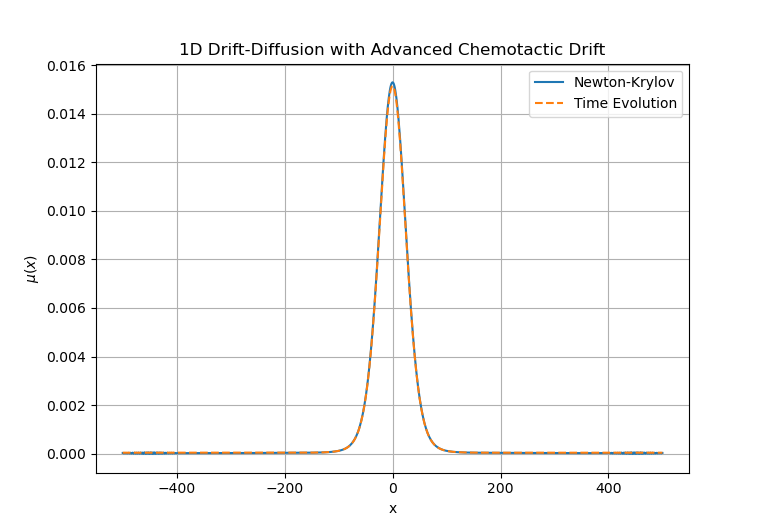
\includegraphics[width=0.8\linewidth]{figures/Advanced Chemotaxis Steady State.png}
    \caption{Steady-state distributions of the advanced chemotaxis model computed by Newton-Krylov (blue) and time evolution (orange).}
    \label{fig:advanced_chemotaxis_ss}
\end{figure}

\begin{figure}[ht]
    \centering
    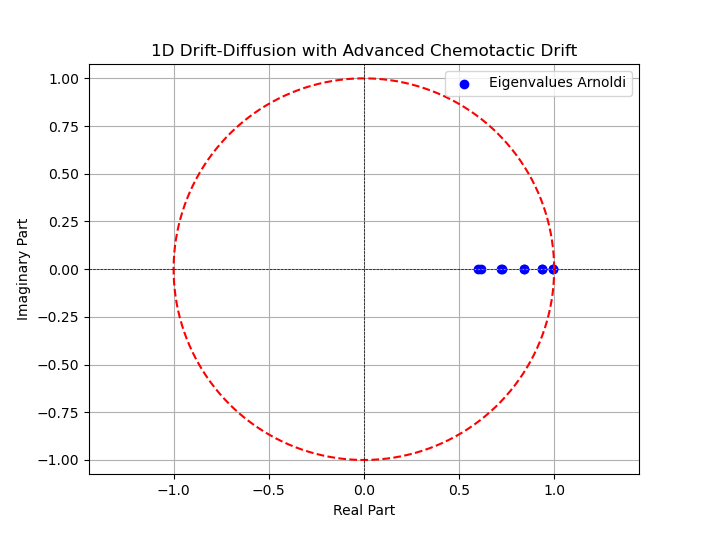
\includegraphics[width=0.8\linewidth]{figures/Advanced Chemotaxis Eigenvalues.png}
    \caption{Leading eigenvalues of the timestepper for the advanced chemotaxis model computed by the Arnoldi method.}
    \label{fig:advanced_chemotaxis_arnoldi}
\end{figure}

\section{Newton-Krylov for Particle Methods}
As we have agreed many times, if $X$ is a collection of particles, then solving
\begin{equation}
    \psi(X) = X - \phi_T(X) = 0
\end{equation}
makes no mathematical sense since particles still, and should, move around in a steady state. There is no reason that the $i$-th particle of $\phi_T(X)$ should be closest to the $i$-th particle in $X$. However, we can make this problem mathematically well defined by minimizing a Wasserstein distance instead. Let $p$ and $q$ be two permutations of the index set $\{1,2,3,\dots,N\}$ so that the re-indexed particles $X_p$ and $\phi_T(X)_q$ are ordered. This is identical to applying the optimal transport map from $X$ to $\phi_T(X)$. Then, one can see that
\begin{equation}
    \psi(X_p)^T \psi(X_p)= \frac{1}{N} \sum_{n=1}^N (X_{p(i)} - \phi_T(X)_{q(i)})^2 = W^2_2(X, \phi_T(X)).
\end{equation}
The correct steady-state objective for particle dynamics is therefore to minimize this Wasserstein distance! In practice, this boils down to an optimization problem in $N$ dimensions. To our surprise, gradient-based optimizers like Adam work really well for this!

\subsection{Algorithm} \label{subsec:particle_algorithm}
In this section, we derive a numerical algorithm to minimize the Wasserstein distance between the coupled particle clouds $X$ and $X(T) = \phi_T(X)$. I heavily relied on ChatGPT-o3 for the math, so it would be good if someone could check for correctness.

The objective function is half of the squared Wasserstein-2 distance $W_2^2(X, \phi_T(X))$
\begin{equation}
    F(X) = \frac{1}{2}W_2^2(X, \phi_T(X))
\end{equation}
The Wasserstein-2 distance is reasonably well behaved, which makes optimization relatively straightforward. Just for self-containedness, the Wasserstein distance between two probability vectors $a, b$ and the associated cost matrix $C_{i,j} = c(X_i, Y_j)$ is defined as the optimal coupling $P$ so that
\begin{equation} \label{eq:regularized_OT_loss}
    W_2(a, b, C) = \underset{P \in \Pi(a,b)}{\min} \left\langle P, C\right\rangle
\end{equation}
In our setting, the vectors $a$ and $b$ are just uniform because they are empirical measures for $X$ and $\phi_T(X)$. The minimization is achieved over all joint probability matrices $P$ such that its marginals are $a$ and $b$ respectively. An advantage of the Wasserstein distance is that it is smooth, easily differentiable with a known gradient, and most importantly, convex.

Interestingly, the gradients of $F$ have a known formula! This makes our computational approach a lot more efficient. For fixed particle ensembles $X$ and $Y$, we have
\begin{align} \label{eq:sinkhorn_div_gradient}
    \nabla_X \frac{1}{2} W_2(X, Y) &= X - P Y \\
    \nabla_Y \frac{1}{2} W_2(X, Y) &= Y - P^T X
\end{align}
where $P$ is the optimal transport plan given by equation~\eqref{eq:ot_plan}. Plugging these two formulas into the gradient of the objective, we obtain
\begin{align} \label{eq:objective_gradient}
\begin{split}
    \nabla_X F(X) &= \nabla_1 \frac{1}{2} W_2^2(X, \phi_T(X)) + \left[D\phi_T(X)\right]^T  \nabla_2 \frac{1}{2} W_2^2(X, \phi_T(X)) \\ &= \underbrace{X - NP \phi_T(X)}_{\text{Part A}} + \underbrace{\left[D\phi_T(X)\right]^T \left(\phi_T(X) - NP^T X\right)}_{\text{Part B}}
\end{split}
\end{align}

When the timestepper $\phi_T$ is stochastic, the Jacobian $D\phi_T(X)$ is not well-defined because it depends on the exact Brownian increments used in the Euler-Maruyama scheme. As a result, this gradient will likely blow up and contain a lot of noise. Therefore, we only use part A in the gradient expression~\eqref{eq:objective_gradient} of $F$ 
\begin{equation}
    \tilde{\nabla} F(X) = \nabla_1 \frac{1}{2} W^2_2(X, \phi_T(X)) = \underbrace{X - NP \phi_T(X)}_{\text{Part A}}
\end{equation}
during optimization. Think of $\tilde{\nabla} F(X)$ as a preconditioner of $\nabla F(X)$. It has already been proposed in the literature, see specifically references~\cite{hunter2004tutorial,razaviyayn2013unified,benamou2015iterative}. Importantly, it can be proven that the Wasserstein distance will decrease monotonously when only using this first part of the gradient. All our numerical results were generated using this truncated / preconditioned gradient. Either way, the gradients are computed numerically through PyTorch, but I make sure to detach $Y = \phi_T(X)$ to avoid the second term. 

Now we can just plug in the objective $F(X)$ and its gradient into any optimization algorithm of our choice and find steady-state distributions of particles methods! We have good results for the Adam optimizer, but the Newton-Krylov method requires some extra work.

\subsection{Stochastic Signal-to-Noise Ratio for Newton-Krylov}
We can also apply the Newton-Krylov method to solve the Wasserstein minimization problem. Instead of minimizing $F(X)$ directly, rather we solve
\begin{equation} \label{eq:particle_nk}
    G(X) = \tilde{\nabla} F(X) = X - NP\phi_T(X) = X - OT(\phi_T(X)) = 0.
\end{equation}
So we want to find the root of $G$, and this is mathematically equivalent to minimizing $F$ or solving $\psi(X) = 0$ but with OT regularization.

Let us have a closer look at the approximation and stochastic errors that appear during Newton-Krylov. Specifically, let us look at the finite-differences approximation of the Jacobian $J(X_k) \cdot v = DG(X_k) \cdot v$ in equation~\eqref{eq:fd}. In our framework, we make a stochastic error on $G$
\begin{equation}
    \tilde{G}(X) = G(X) + \frac{\sigma}{\sqrt{N}} \xi
\end{equation}
where $\xi$ is a standard normally distributed number. Then, the finite differences approximation becomes
\begin{align}
    \tilde{J}(X_k) v &\approx \frac{\tilde{G}(X_k + \varepsilon v) - \tilde{G}(X_k)}{\varepsilon}  \\ &= \frac{G(X_k + \varepsilon v) + \frac{\sigma}{\sqrt{N}} \xi_1 - G(X_k) -  \frac{\sigma}{\sqrt{N}} \xi_2}{\varepsilon} \\
    &= \frac{G(X_k + \varepsilon v) - G(X_k)}{\varepsilon} + \frac{\sigma}{\varepsilon \sqrt{N}}(\xi_1 - \xi_2). \\
    &= J(X_k) \cdot v + \mathcal{O}\left(\varepsilon + \frac{\xi_1 - \xi_2}{\varepsilon \sqrt{N}} \right)
\end{align}
The stochastic error term
\begin{equation}
    \frac{\sigma}{\varepsilon \sqrt{N}}(\xi_1 - \xi_2)
\end{equation}
is normally distributed with zero mean and standard deviation $ \frac{\sqrt{2}\sigma}{\varepsilon \sqrt{N}}$. The $\varepsilon$ in the denominator can really blow this thing up if its value is not chosen carefully!

Since this is the intrinsic accuracy of our function $\tilde{\psi}$, it only makes sense that we choose the GMRES tolerance $\delta$ to be on the same level, i.e., 
\begin{equation}
    \delta = \mathcal{O}\left(\varepsilon + \frac{1}{\varepsilon \sqrt{N}}\right)
\end{equation}
Combining this result with the estimate of the forward accuracy of Newton-Krylov~\eqref{eq:nk_accuracy}, we obtain
\begin{equation}
    \norm{X_{\infty} - X^*} \leq C \norm{J(X^*)^{-1}} \left( 
 \varepsilon + \frac{1}{\varepsilon \sqrt{N}} + \text{rounding errors}\right)
\end{equation}
(There should be an expected value somewhere, but I don't really care at this point.) This estimate further underlines the point that $\varepsilon$ and $N^{-1/2}$ should be of the same order of magnitude.

\subsection{Numerical Results for the Simple Chemotaxis Example}
I implemented the Adam optimizer on the objective that we discussed in Section~\ref{subsec:particle_algorithm} on the simple chemotaxis model. The setup is as follows. The initial particles are distributed according to a standard Gaussian measure (blue histogram on Figure~\ref{fig:wasserstein_adam}) and we ran the Adam optimizer for 300 epochs. We applied an adaptive learning rate schedule by starting at a learning rate of $10^{-1}$ and decreasing it by a factor $10$ every $50$ epochs. We do not use minibatching. Important to note is that the integration horizon of the timestepper $\phi_T$ is $T = 1s$.

Figure~\ref{fig:wasserstein_loss} (blue curve) shows the per-epoch Wasserstein distance on a logarithmic scale. We also show the loss gradient in orange. After an initial drop of three orders of magnitude, the curve levels off around~$5\times10^{-5}$. The orange curve plots the $\ell^{2}$–norm of the gradient; it decays in lockstep with the loss and then stagnates in the same narrow band.

\begin{figure}[ht!]
    \centering
    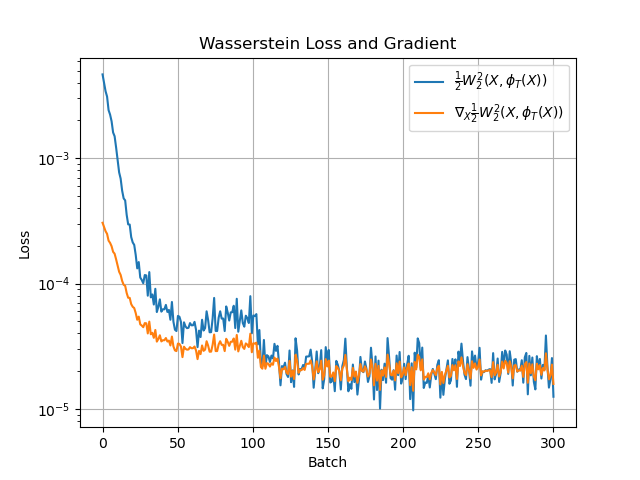
\includegraphics[width=0.8\linewidth]{figures/Wasserstein_Adam_Loss_Convergence.png}
    \caption{Wasserstein loss at each optimization epoch. We note convergence to about $5\times10^{-6}$, which is close to the single-precision machine precision of my GPU.}
    \label{fig:wasserstein_loss}
\end{figure}

Figure~\ref{fig:wasserstein_adam} compares the optimized particle histogram (orange bars) to the analytic steady‐state density (red dashed line). We can clearly see an almost perfect match between the optimized particle distribution and the true steady-state (invariant) distribution. Important to note is that this convergence already happens after about $100$ epochs (that is when the loss stagnates in~\ref{fig:wasserstein_loss}. This number of epochs corresponds to a total integration time of $100s$ because $T = 1s$. Said differently, we can reach the steady state faster than through regular time evolution (500 seconds). 

\begin{figure}[ht]
    \centering
    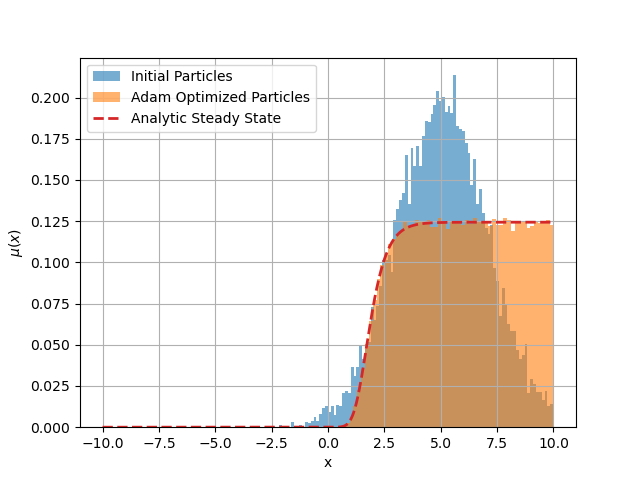
\includegraphics[width=0.8\linewidth]{figures/Wasserstein_Adam_Histograms.png}
    \caption{Adam-optimized particles (orange) compared with the analytic steady-state density (dashed green). The initial particles are also shown in blue.}
    \label{fig:wasserstein_adam}
\end{figure}

The particle Newton-Krylov algorithm~\eqref{eq:particle_nk} does not work well. Figure~\ref{fig:nk_particles} shows the particle distribution after $100$ Newton-Krylov steps. Figure~\ref{fig:nk_residual} further shows the residual of~\eqref{eq:particle_nk} as a function of the Newton iteration number. We observe no convergence at all. The residual remains at a constant high level (compared to Figure~\ref{fig:wasserstein_loss}) and the final particle distribution is very similar to the initial distribution.

\begin{figure}[ht]
    \centering
    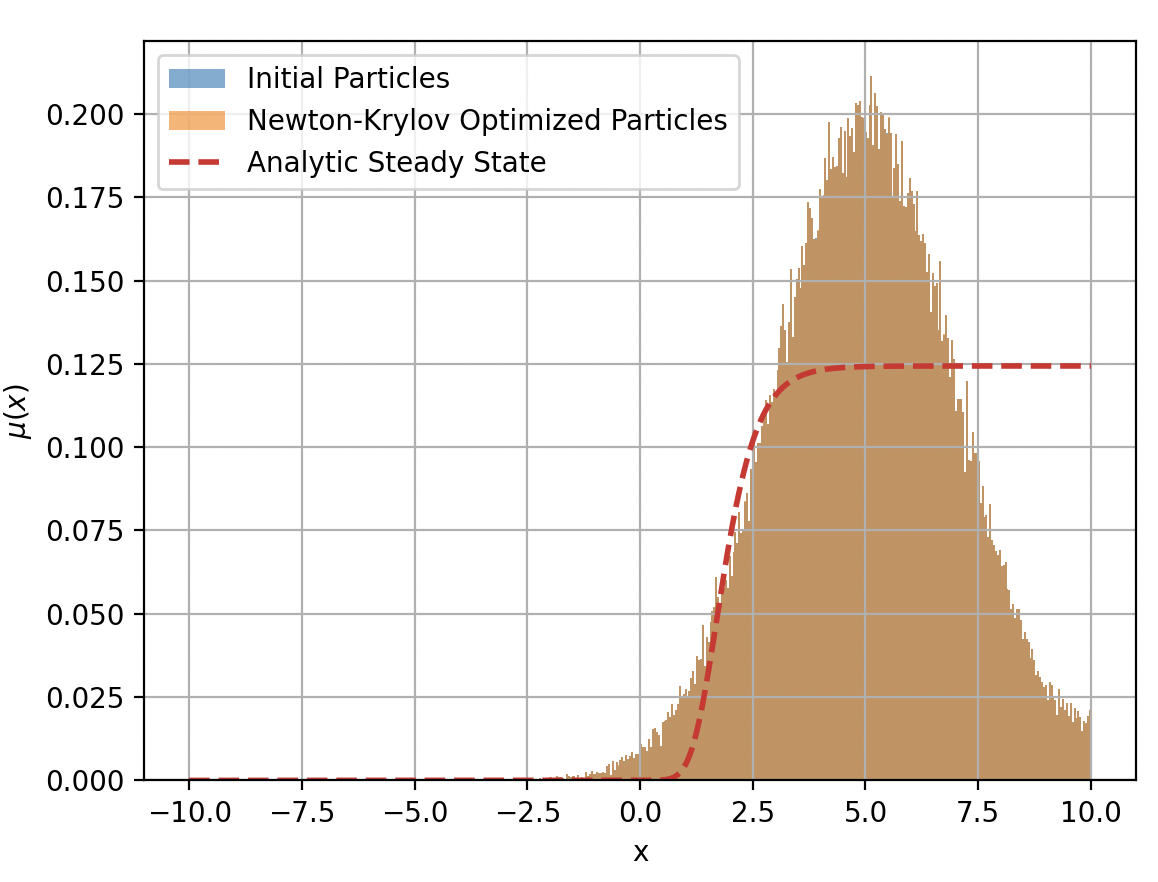
\includegraphics[width=0.7\linewidth]{figures/Simple Chemotaxis NK Particles.png}
    \caption{Newton-Krylov-optimized particles (orange) compared with the analytic steady-state density (dashed green). The initial particles are also shown in blue.}
    \label{fig:nk_particles}
\end{figure}

One might ask why the Adam optimizer converges well, but the Newton-Krylov solver does not. The reason for this dichotomy is that Adam and Newton-Krylov are solving different objectives with different degrees of regularity / smoothness. On the one hand, the Adam optimizer explicitly minimizes the Wasserstein distance~\eqref{eq:regularized_OT_loss} which is a differentiable function in the particle positions. On the other hand, the Newton method attempts to solve the same problem by solving the gradient equation~\eqref{eq:particle_nk} which is not differentiable in the (stochastic) particle positions. The Newton-Krylov method requires more smoothness than is present in the Wasserstein / gradient formulation, and therefore there is no meaningful information that can be extracted from the Newton search direction $\nabla G(x_k)^{-1} G(x_k)$. Our hypothesis is that these search vectors point in random directions, and there is no movement in $x_k$ on average.

\begin{figure}[ht]
    \centering
    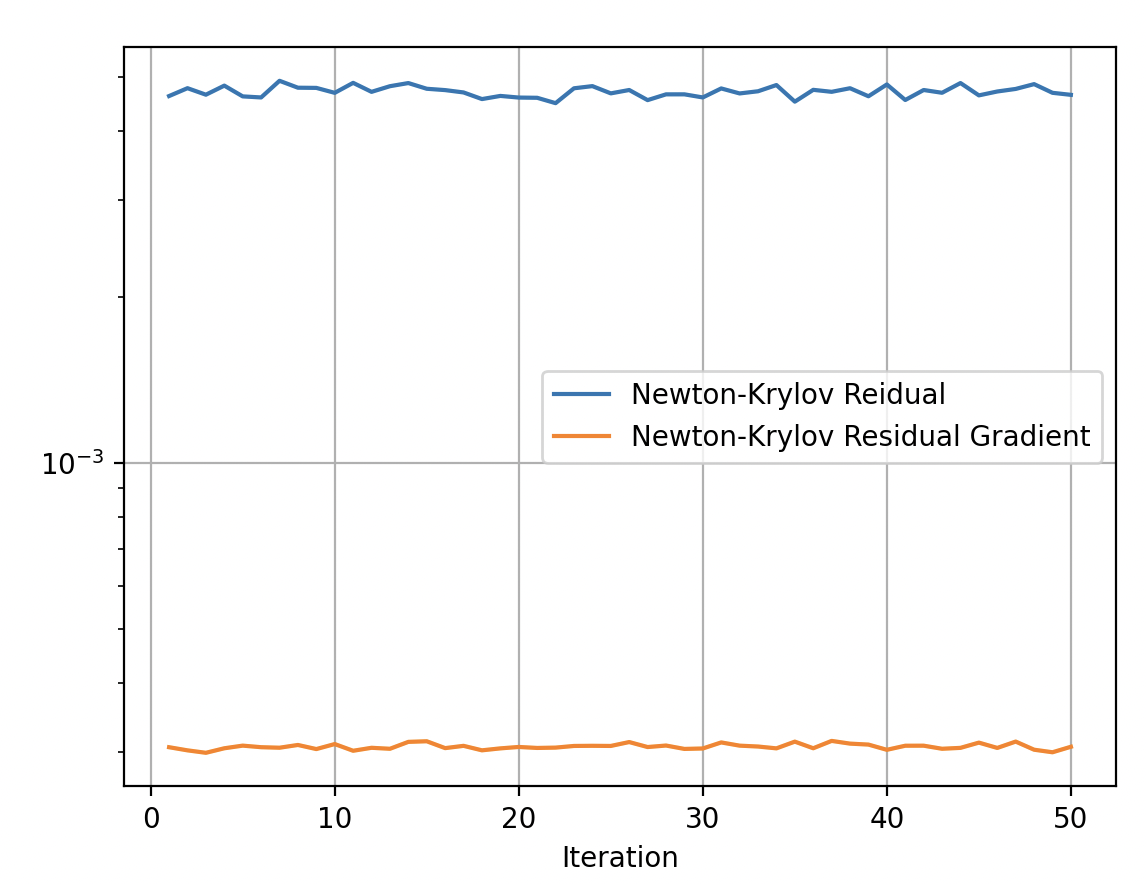
\includegraphics[width=0.7\linewidth]{figures/Residual NK Particles.png}
    \caption{Newton-Krylov residual (blue) and its gradient (orange) as a function of the iteration number}
    \label{fig:nk_residual}
\end{figure}

\subsection{From Particles to Densities}
We have shown in the previous section that minimizing the Wasserstein distance between two particle clouds at different times leads to the invariant or steady-state distribution when using the correct optimizer. The Adam optimizer only uses Wasserstein-gradient information, and we can correctly recover the steady state, but the Newton-Krylov solver is unable to do so, presumably because the problem of $\tilde{\nabla} \frac{1}{2} W_2^2 = 0$ is not well-enough defined. This observation begs the following obvious question: Can we increase the regularity of the particle-to-particle timestepper enough to make Newton-Krylov work? Turns out the answer is yes! We explore the use of probability density functions in this section, and the smoother alternative of cumulative density functions (CDF) in the next.

We can create a density-to-density timestepper or mapping using the lifting and restriction operators from the equation-free framework. The main idea is that we keep track of the current density $\mu_k(x)$ in a number of fixed grid points $\{x_m\}_{m=1}^M$. Evaluating $\mu_k$ in these grid points leads to a vector $\rho_k \in \mathbb{R}^M$. We can ensure that $\rho_k$ is always normalized by simply rescaling.  Starting from the current density $\rho_k(x)$, we can construct the density at some later time $T$ in three steps: i) Sample $N$ particles $X$ from $\rho_k$ using any MCMC routine (lifting); ii) Propagate the particles over a time window of size $T$ to obtain $\phi_T(X)$; iii) Compute the new density $\rho_{k}(T)$ of $\phi_T(X)$ using Gaussian kernel density estimation (restriction). The end result of these three steps is a mapping
\begin{align} \label{eq:density_timestepper}
    \varphi_T: \ &\mathbb{R}^M \to \mathbb{R}^M \\
    &\rho_k \mapsto \varphi_T(\rho_k).
\end{align}
We can then define our root function in the same way, $\psi(\rho) = \rho - \varphi_T(\rho)$, and steady states again correspond to $\psi(\rho) = 0$.

Before showing the numerical results, let us look at the lifting and restriction steps in more detail. Lifting creates particles from densities. We cannot assume much structure on $\mu_k$ or its representation $\rho_k$, so we can only sample it using Markov chain Monte Carlo. In the following experiment, I implemented a Hamiltonian Monte Carlo (HMC) sampler with a step size so that the averaged acceptance rate is $23\%$ (this is optimal, but the exact step size has to be determined experimentally). I sample $N=10^5$ particles every lifting step. We achieve restriction through Gaussian KDE. The `bandwidth' $\sigma$ or the standard deviation of the Gaussian is an important parameter and must also be determined numerically. I found that the results depend heavily on the choice of bandwidth. You can find more information about Gaussian KDE here, but I created a very fast KDE routine in one dimension using the FFT. 

Let's apply Newton-Krylov to $\psi(\rho) = 0$ on the simple chemotaxis problem. From experimentation, we found that the optimal HMC time step $\Delta t=2$ and that the KDE bandwidth should be $\sigma = 0.01$. We also found that the optimal finite differences step size is $\varepsilon \approx 10^{-1}$ - so, pretty large. We ran $50$ iterations of Newton-Krylov with Wolfe line search, and the results are shown in Figure~\ref{fig:density_convergence}. 

\begin{figure}[ht]
    \centering
    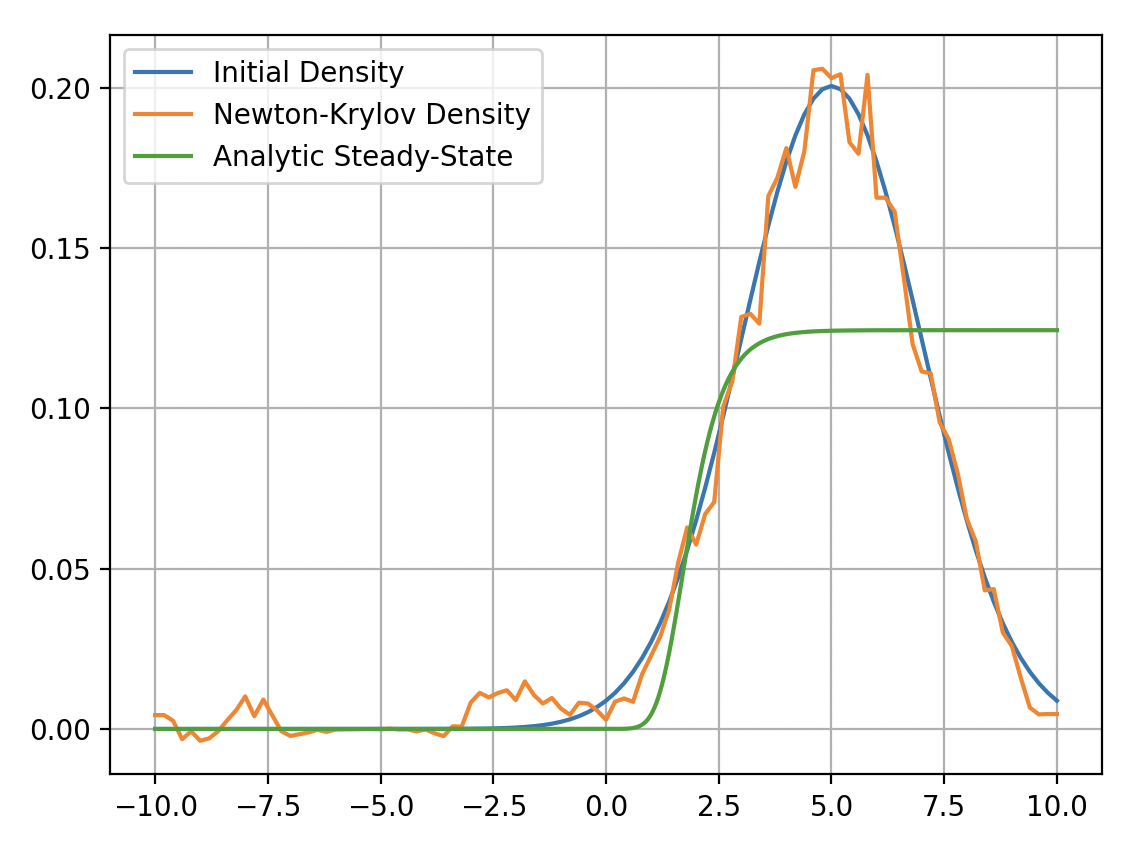
\includegraphics[width=0.7\linewidth]{figures/Simple Chemotaxis Density.png}
    \caption{Newton-Krylov final density (orange) compared with the analytic steady-state (green). The initial density is also shown in blue. The result by Newton-Krylov is very noise and fluctuates around the initial. We observed to convergence towards the steady-state distribution.}
    \label{fig:density_convergence}
\end{figure}

The numerical results are not great. The figure essentially shows that Newton-Krylov is unable to make progress from the initial distribution, even after 50 steps. I believe that the main reason for non-convergence is that estimated densities are inherently too noisy. This is, in my opinion, due to both MCMC and KDE. First of all, MCMC generates correlated particles. This in itself is not a problem, but it might result in some regions being oversampled and others being undersampled. A much bigger reason, however, is the bandwidth parameter in KDE. We can increase regularity by increasing the bandwidth, but then this approach is unable to capture the sharp increase at $x \approx 1$. We observed this numerically. This means the bandwidth must be chosen on the smaller side, which makes the estimated density noisy. This problem is aggravated when there are undersampled/oversampled regions.

For these reasons, we propose to apply the Newton-Krylov method on cumulative density functions instead.

\subsection{Adding Smoothness: From Particles to Cumulative Density Functions}
Cumulative density functions (CDF) are an alternative representation of densities. They are defined as the integral of a density $\mu$
\begin{equation} \label{eq:cdf}
    F(x) = \int_{-\infty}^x \mu(y) dy
\end{equation}
so continuous differentiability is guaranteed. There is a question whether we need to evaluate the CDF in a fixed grid, or simply apply the inverse CDF to obtain sorted (optimally transported) particles. Suppose $X$ is a particle ensemble and $\phi_T$ is the particle timestepper. Then the inverse CDF approach computes
\begin{equation} \label{eq:inverse_cdf}
    X - F^{-1}\left(F\left(\phi_T(X)\right)\right) = X - OT(\phi_T(X)) = G(X)
\end{equation}
where $G$ is the $\psi$-function defined in~\eqref{eq:particle_nk}. We know experimentally, and with theoretical justification, that Newton-Krylov for solving $G(X) = 0$ does not work well due to reduced smoothness.

For this reason, we must evaluate the CDFs on a fixed grid. We define a CDF-to-CDF timestepper $\Phi_T$ similar to our approach with densities~\eqref{eq:density_timestepper} using lifting, particle propagation, and restriction:
\begin{itemize}
    \item[] \textit{Lifting} creates a particle ensemble from the CDF. This is usually done by finding the percentiles of the distribution. If we need $N$ particles, we need to find the locations of the $n / N$-percentile, or solve
    \begin{equation} \label{eq:percentile}
        F(X_n) = \frac{n}{N}, n = 1, \dots, N.
    \end{equation}
    Then, the resulting particle ensemble $X = \{X_n\}_{n=1}^N$ is guaranteed to be distributed according to $F$. Any fast root-finding algorithm for solving~\eqref{eq:percentile} will do. I used the \textit{Brentq} algorithm due to its fast and stable bisection approach. 
    
    There is one complication: $F$ is only known in a number of grid points, and $N$ (the number of particles) is typically much larger than $M$ (the number of grid points). This means we need to approximate $F$ in between the grid points to solve~\eqref{eq:percentile}. From my experience, cubic splines work really well for this because construction, evaluation and differentiation are very fast. We can therefore solve for the percentiles for very little extra work.

    \item[] \textit{Restriction} can be done by applying the definition of a CDF~\eqref{eq:cdf}. Let $x_m$ be the $m$-th grid point, then $F(x_m)$ can be computed as the fraction of the number of particles that are to the left of $x_m$, i.e.
    \begin{equation}
        F(x_m) = \frac{\#\{n \mid X_n \leq x_m\}}{N}
    \end{equation}
\end{itemize}
These two steps combined with $\phi_T$ define a CDF timestepper
\begin{align} \label{eq:cdf_to_cdf}
    \Phi_T: \ &\mathbb{R}^M \to \mathbb{R}^M \\
    &F \mapsto \Phi_T(F).
\end{align}
and we can find steady-state CDFs by solving $\psi(F) = F - \Phi_T(F) = 0$. An advantage of the CDF approach is that there are no parameter choices except for the step size in the Newton-Krylov method. This reduces the complexity by a lot!

\begin{figure}[ht]
    \centering
    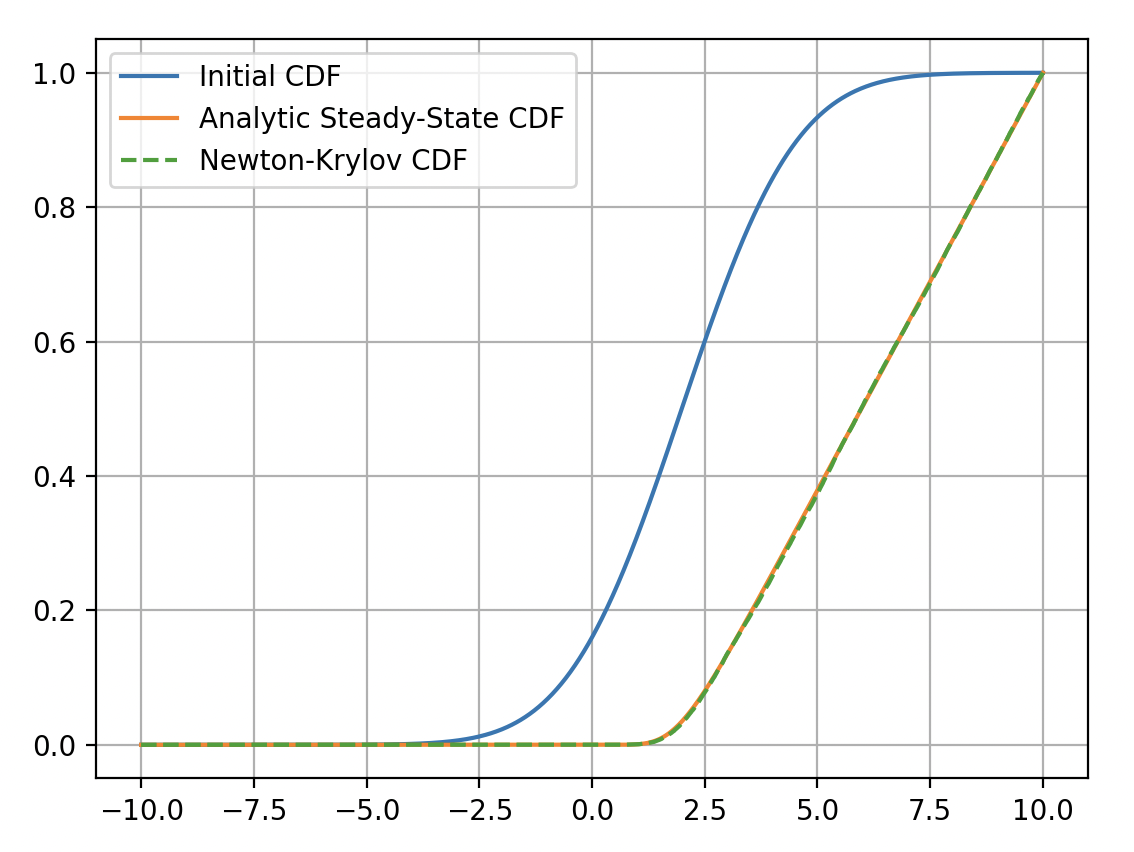
\includegraphics[width=0.7\linewidth]{figures/Simple Chemotaxis CDF.png}
    \caption{Newton-Krylov CDF (dashed orange) compared with the analytic steady-state CDF (green). The initial CDF is also shown in blue.}
    \label{fig:cdf_convergence}
\end{figure}

Figure~\ref{fig:cdf_convergence} shows the result from applying Newton-Krylov with $\varepsilon = 10^{-1}$ to $\psi(F)$. There is fast convergence to the true steady-state CDF in green. The initial CDF of a Gaussian is shown in blue. Note how smooth the optimized CDF is. We also plot the loss ($\norm{\psi(F)}$) per Newton-Krylov iteration / epoch in Figure~\ref{fig:cdf_losses}. This loss decreases fast in the first few iterations and then stagnates near the noise level after about 10 iterations. This inherent noise level is due to the particle timestepper.

\begin{figure}[ht]
    \centering
    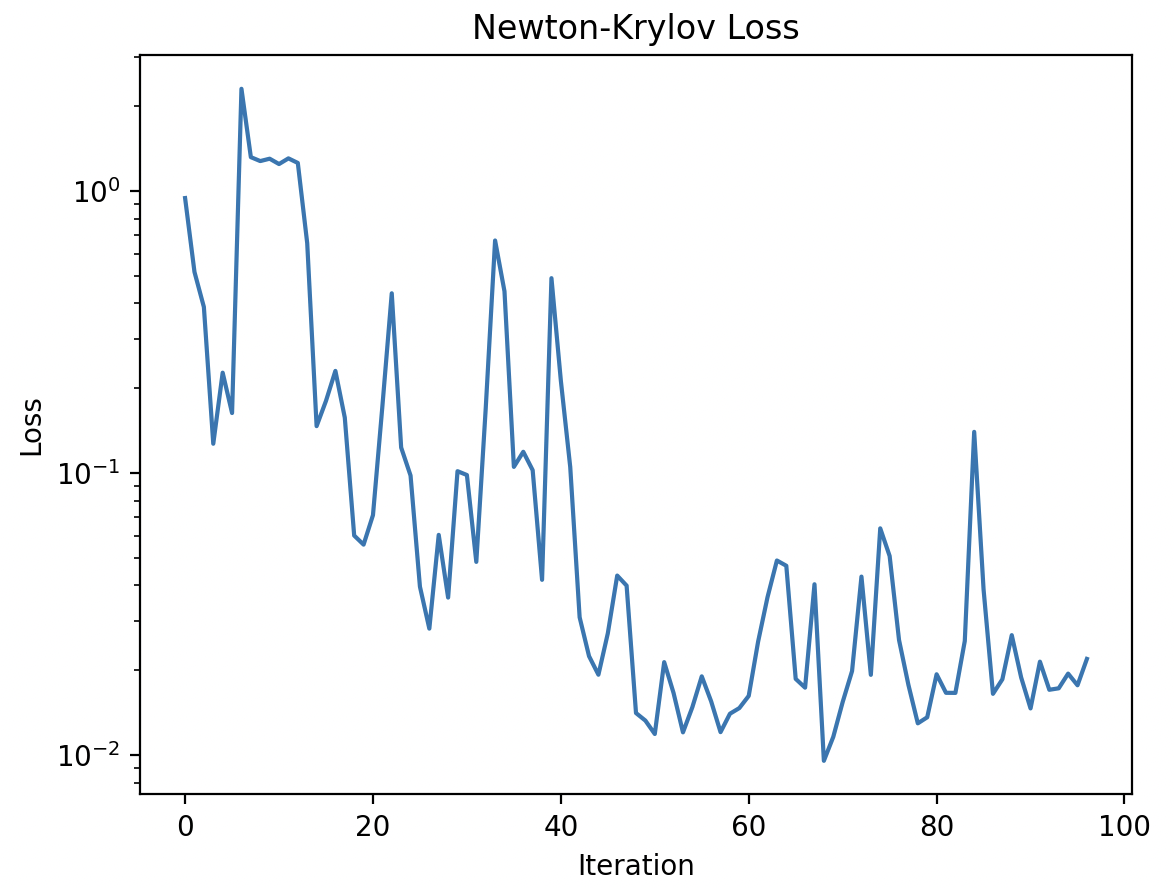
\includegraphics[width=0.7\linewidth]{figures/CDF to CDF NK Losses.png}
    \caption{Residual ($\norm{\Psi(F_k)}$ of Newton-Krylov applied to the CDF to CDF timestepper~\eqref{eq:cdf_to_cdf} as a function of the Newton iteration number $k$. We see a steady but chaotic decrease to the noise level of approximately $2 \cdot 10^{-2}$.}
    \label{fig:cdf_losses}
\end{figure}

I will make a plot of the loss as a function of $\varepsilon$ to determine the optimal finite-difference step size next. Afterwards, we should move on to a two-dimensional example.

\subsection{Expanding CDFs to Multiple Dimensions}
The algorithm that we created in the previous section is inherently one-dimensional because percentiles are only well-defined in one dimension. However, the concept of a cumulative density can be extended to multiple dimensions. For example, in 2D, we can simply define the CDF
\begin{equation} \label{eq:cdf_2d}
    F_{X,Y}(x, y) = P\left(X \leq x \ \text{and} \ Y \leq y\right) = \int_{-\infty}^x \int_{-\infty}^y p(u, v) du dv,
\end{equation}
where $p_{X,Y}(u, v)$ is the two-dimensional density of the particles $(X,Y)$. We explicitly add the subscript $X,Y$ to the CDF and density because we can also define marginal and conditional CDFs. These two concepts are crucial to sampling using CDFs in multiple dimensions. First of all, we can define the marginal CDF of $X$ as just the cumulative density function of $X$ by integrating over the $Y$ direction.
\begin{equation} \label{eq:marginal_cdf}
    F_X(x) = P\left(X \leq x\right) = P\left(X \leq x \ \text{and} \ Y \leq \infty\right) = F_{X,Y}(x, \infty)
\end{equation}
This is identical to~\eqref{eq:cdf}. Similarly, we can define the conditional CDF of $Y$ for a specific value of $X = x$ as the CDF of the marginal density function,
\begin{equation}
    p_{Y|x}(y) = \frac{p_{X,Y}(x, y)}{p_X(x)}
\end{equation}
where $p_X(x)$ is the marginal distribution of $X$. Then, the conditional CDF reads
\begin{equation}
    F_{Y|x}(y) = P\left(Y \leq y \mid X = x\right) = \int_{-\infty}^y p_{Y|x}(v) dv = \int_{-\infty}^y \frac{p_{X,Y}(x, v)}{p_X(x)} dv
\end{equation}
It is well known from elementary probability theory that this marginal CDF can be alternatively written as
\begin{equation} \label{eq:conditional_cdf}
    F_{Y|x}(y) = \frac{\partial_x F_{X,Y}(x,y)}{p_X(x)}
\end{equation}

The last equation especially suggests a fast algorithm to put samples at the 'percentiles' of a two-dimensional CDF. We will again evaluate the CDF on a fixed grid. The algorithm proceeds as follows: 1) Given the values of the 2D CDF in the grid, build an interpolating spline that approximates the 2D surface; 2) Build the marginal CDF~\eqref{eq:marginal_cdf} as a restriction of the 2D spline to $y = \infty$ (or its maximum value); 3) Put $N_x$-samples $x_p$ at the percentiles of the marginal CDF (can be done fast!); 4) Compute the partial derivative in the $x-$ direction at every value of $x_p$ and at every grid point in $y$. This operation must only be done once and is fast due to the nature of splines and vectorized operations; 5) For every $x_p$, construct the conditional CDF~\eqref{eq:conditional_cdf} and put $N_y$ samples at its percentiles. This algorithm correctly generates $N_x N_y$ samples from the joint distribution $p_{X,Y}$. I believe a version of this algorithm was already proposed in~\cite{zou2005equation} but it was never written down explicitly. By leveraging the fast construction of splines and its derivatives, we can easily generate $10^5$ to $10^6$ samples in about $30$ milliseconds.

I implemented the multidimensional CDF algorithm on a 2D half-moon potential. The stochastic microscopic dynamics is given by the overdamped Langevin equation
\begin{equation}
    dX = -\nabla U(X) dt + \sqrt{2} dW,
\end{equation}
where $X = (x, y) \in \mathbb{R}^2$, $W$ is Brownian motion and the potential energy $U(X)$ is defined as
\begin{equation} \label{eq:half_moon_potential}
    U(x, y) = A (r - R)^2 + B \exp\left(-\alpha (y - y_0)\right)
\end{equation}
with $r = \sqrt{x^2 + y^2}, A = 2.0, B = 0.5, R = 2.0, \alpha=1.5,$ and $y_0 = -0.5$. A three-dimensional view of the associated invariant distribution $\propto \exp\left(-U(x, y)\right)$ is shown in Figure~\ref{fig:halfmoonpotential}.
\begin{figure}
    \centering
    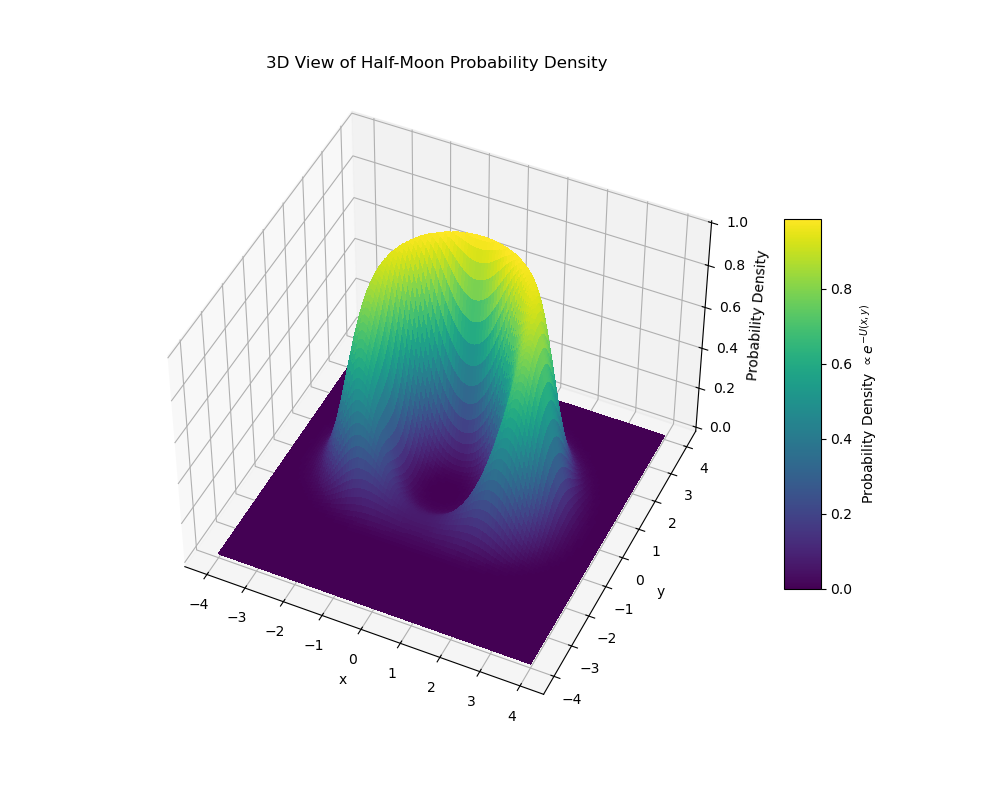
\includegraphics[trim={0.5cm 2cm 0.5cm 2cm},width=0.9\linewidth]{figures/half_moon_potential.png}
    \caption{A three-dimensional view of the invariant distribution associated to the half-moon potential~\eqref{eq:half_moon_potential}.}
    \label{fig:halfmoonpotential}
\end{figure}
The steady-state found by the particle Newton-Krylov method is shown in Figure~\ref{fig:NK_2d_results}. At each iteration, we sample the 2D CDF using $10^6$ particles, evolve the particles through the overdamped Langevin equation over a horizon of $T = 1s$ with time steps of size $\delta t = 10^{-3}$, and restrict the CDF back on a uniform grid of $100 \times 100$. Through experimentation, we found that $\varepsilon = 0.1$ is near-optimal.

As one can see in Figure~\ref{fig:nk_2d_loss} it can take a while before the Newton-Krylov solver converges to the steady state because the loss landscape is very noisy. In my experience, Newton-Krylov always does find the steady-state distribution, sometimes immediately, but sometimes only after bouncing around for $50$ epochs. The noise level for this example seems to be $\norm{\psi(X)} \approx 6 \times 10^{-2}$.
\begin{figure}
    \centering
    \begin{subfigure}[t]{0.5\linewidth}
        \centering
        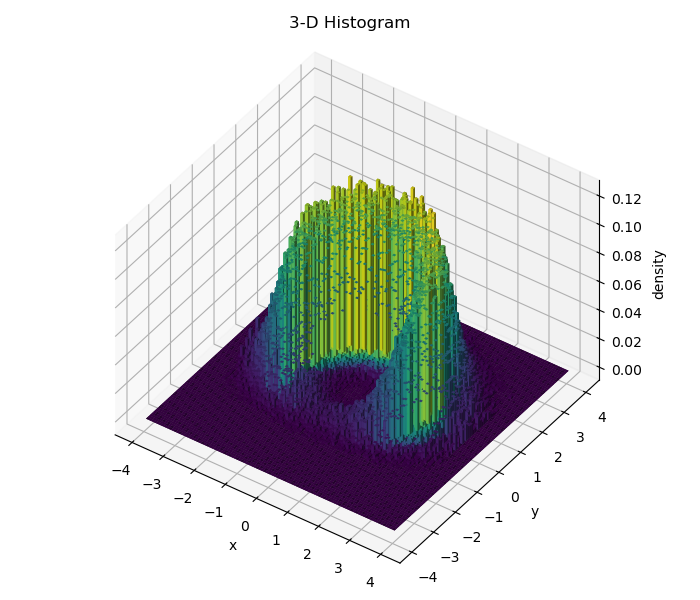
\includegraphics[width=\linewidth]{figures/NK_3d_view.png}
    \end{subfigure}%
    \begin{subfigure}[t]{0.5\linewidth}
        \centering
        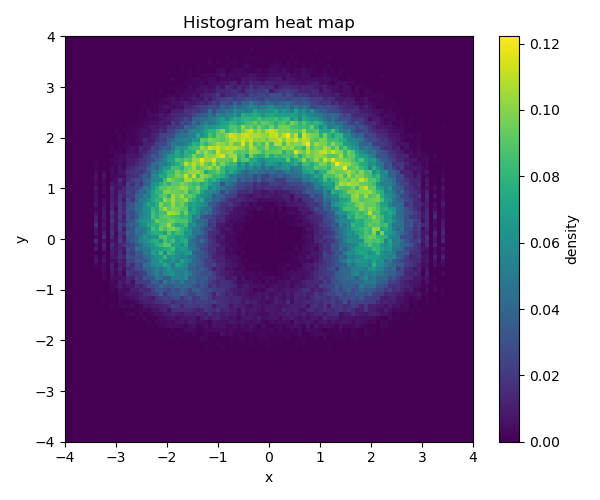
\includegraphics[width=\linewidth]{figures/NK_2d_view.png}
    \end{subfigure}
\caption{(Left) Three-dimensional view of the particle histogram obtained by the Newton-Krylov optimizer; (Right) Two-dimensional heat map of the same histogram.}
\label{fig:NK_2d_results}
\end{figure}

\begin{figure}
    \centering
    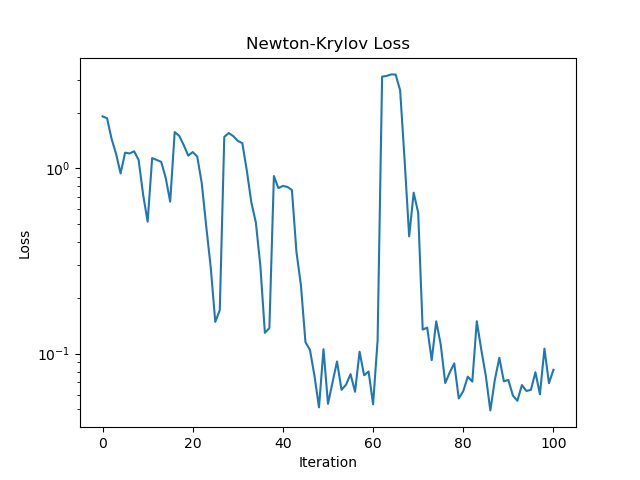
\includegraphics[width=0.75\linewidth]{figures/NK_2D_loss.png}
    \caption{Loss $\norm{\psi(X_k)}$ at each iteration of the Newton-Krylov method. It takes a while for the solver to converge, but eventually it does at the noise level of $6 \times 10^{-2}$.}
    \label{fig:nk_2d_loss}
\end{figure}

\section{Invariant Distribution from Trajectories}
Suppose we have a system of particles governed by a stochastic differential equation
\begin{equation}
    dX = -\nabla U(X)dt + \sqrt{2} \beta^{-1} dW
\end{equation}
where $U(x)$ is a potential energy function, $dW$ is Brownian Motion and $\beta$ is the inverse temperature of the system. The invariant distribution is fully determined by the potential energy 
\begin{equation}
    \mu(dx) \propto \exp\left(-\beta U(x)\right)dx.
\end{equation}
Furthermore, ignoring the Brownian motion for now, the particle trajectories are principally determined by the force $F(x) = -\nabla U(x)$, or the gradient of the potential. This begs the question if we can estimate $U(x)$, and by extension $\mu(x)$, from measured trajectories alone?

Let $X = \{X_n\}_{n=1}^N$ be a particle ensemble at time $t = 0$ and let $Y = \{Y_n\}_{n=1}^N = \phi_{\Delta t}(X)$ the time-evolved particles at some later time $\Delta t$. When $\Delta t$ is small (hence we use the notation $\Delta t$ instead of $T$), then each particle difference follows a normal distribution
\begin{equation} \label{eq:normal_trajectories}
    Y_n - X_n \sim \mathcal{N}\left(-\nabla U(X_n) \Delta t, \ 2 \beta^{-1} \Delta t I_d \right)
\end{equation}
where $I_d$ is the unit matrix. We can build an estimator for the potential energy $U(x)$ by writing it as a linear combination of basis functions $\psi_p$. This ansatz reads
\begin{equation} \label{eq:ansatz}
    U_\theta(x) = \sum_{j=1}^p \theta_j \psi_j(x)
\end{equation}
where $\theta \in \mathbb{R}^p$. We can also write down the gradient of the potential as
\begin{equation}
    \nabla U_\theta(x) = \sum_{j=1}^p \theta_j \nabla \psi_j(x)
\end{equation}
Combining this ansatz with the approximate normal distribution for the trajectories~\eqref{eq:normal_trajectories}, we can write down a minimum-likelihood estimator
\begin{equation}
    \theta^* = \underset{\theta \in \mathbb{R}^p}{\arg \min} - \frac{\beta}{4 \Delta t}\frac{1}{N} \sum_{n=1}^N \norm{Y_n - X_n + \Delta t \sum_{j=1}^p \theta_j \nabla \psi_j(X_n) }^2
\end{equation}
In practice, we solve a linear system
\begin{equation}
    G_N \theta^* = b_n
\end{equation}
with
\begin{align*}
    G_N &= \frac{1}{N} \sum_{n=1}^N \nabla \psi(X_n) \nabla \psi(X_n)^T \\
    b_N &= -\frac{1}{N} \sum_{n=1}^N \nabla \psi(X_n) \frac{Y_n - X_n}{\Delta t}.
\end{align*}
In the above equations, we use the notation $\psi = \left(\psi_1, \psi_2, \dots, \psi_p\right)$. Putting the optimal parameters $\theta^*$ together with the functional form~\eqref{eq:ansatz}, we can write an estimator for the potential energy and the invariant density
\begin{align*}
    U_{\theta^*}(x) &= \sum_{j=1}^p \theta^*_j \psi_j(x) \\
    \mu_{\theta^*}(x) &= \propto \exp\left(-\beta U_{\theta^*}(x)\right).
\end{align*}

\paragraph{A note on the basis functions} A popular choice for the basis functions $\psi_j$ are radial basis functions (RBFs) centered at fixed collocation points $x_j$. Radial basis functions are of the form
\begin{equation}
    \psi_j(x) = \exp\left(-\frac{(x - x_j)^2}{2 \sigma^2}\right)
\end{equation}
and they typically work very well for general function approximations. I prefer them for this reason. There is one caveat: our approximation $U_{\theta^*}(x)$ will converge to $0$ as $|x| \to \infty$, while the actual potential energy will diverge to infinity. We will still get a good approximation of the true potential outside this limiting regime, but it is a conceptual problem. I think we need to add one basis function $\psi_0(x) = \frac{1}{2} x^2$ to ensure divergence to infinity for large $x$. What do you think?


\bibliographystyle{plain}
\bibliography{references.bib}
\end{document}
